% ============================================================================
%  Rapport de projet - Simulation discrète d'une caisse de retraite
%  Compilation : pdflatex rapport.tex (x2 pour la table des matieres)
%  ou           : latexmk -pdf rapport.tex
% ============================================================================

\documentclass[12pt,a4paper,oneside]{report}

% --- Encodage et langue --------------------------------------------------
\usepackage[utf8]{inputenc}
\usepackage[T1]{fontenc}
\usepackage[french]{babel}
\usepackage{lmodern}

% --- Mise en page --------------------------------------------------------
\usepackage[a4paper,top=2.5cm,bottom=2.5cm,left=2.5cm,right=2.5cm]{geometry}
\usepackage{setspace}
\onehalfspacing
\usepackage{parskip}
\setlength{\parindent}{0pt}
\setlength{\parskip}{0.6em}

% --- Couleurs et titres --------------------------------------------------
\usepackage{xcolor}
\definecolor{primary}{HTML}{0F4C81}
\definecolor{accent}{HTML}{00A39A}
\definecolor{darkgray}{HTML}{2C3E50}
\definecolor{lightgray}{HTML}{ECF0F1}
\definecolor{codegray}{HTML}{F4F6F8}

\usepackage{titlesec}
\titleformat{\chapter}[display]
  {\normalfont\huge\bfseries\color{primary}}
  {\chaptertitlename\ \thechapter}{20pt}{\Huge}
\titleformat{\section}{\Large\bfseries\color{primary}}{\thesection}{1em}{}
\titleformat{\subsection}{\large\bfseries\color{darkgray}}{\thesubsection}{1em}{}
\titleformat{\subsubsection}{\normalsize\bfseries\color{darkgray}}{\thesubsubsection}{1em}{}

% --- Liens, refs, bibliographie ----------------------------------------
\usepackage[hidelinks,colorlinks=true,linkcolor=primary,urlcolor=accent,citecolor=accent]{hyperref}
\usepackage{cleveref}

% --- Mathematiques ------------------------------------------------------
\usepackage{amsmath,amssymb,mathtools}

% --- Graphismes ---------------------------------------------------------
\usepackage{graphicx}
\usepackage{float}
\usepackage{subcaption}
\graphicspath{{../resultats/}{figures/}}

% --- Tableaux -----------------------------------------------------------
\usepackage{booktabs,array,longtable,tabularx,multirow}
\usepackage{colortbl}
\renewcommand{\arraystretch}{1.25}

% --- Code source --------------------------------------------------------
\usepackage{listings}
\lstdefinestyle{pythonstyle}{
    language=Python,
    backgroundcolor=\color{codegray},
    basicstyle=\ttfamily\footnotesize,
    keywordstyle=\color{primary}\bfseries,
    stringstyle=\color{accent},
    commentstyle=\color{darkgray}\itshape,
    numbers=left,
    numberstyle=\tiny\color{gray},
    stepnumber=1,
    numbersep=8pt,
    showstringspaces=false,
    breaklines=true,
    frame=single,
    rulecolor=\color{lightgray},
    captionpos=b,
    tabsize=4,
}
\lstset{style=pythonstyle}

% --- En-tetes et pieds de page -----------------------------------------
\usepackage{fancyhdr}
\pagestyle{fancy}
\fancyhf{}
\fancyhead[L]{\nouppercase\leftmark}
\fancyhead[R]{\thepage}
\fancyfoot[C]{\small Simulation discrete -- Caisse de retraite marocaine}
\renewcommand{\headrulewidth}{0.4pt}

% --- Macros utiles ------------------------------------------------------
\newcommand{\dhe}{\,\textit{DH}}
\newcommand{\mdhe}{\,\textit{Mdhs}}
\newcommand{\code}[1]{\texttt{\color{primary}#1}}

% ============================================================================
\begin{document}

% ----- PAGE DE GARDE ----------------------------------------------------
\begin{titlepage}
\begin{center}
\vspace*{0.5cm}

{\Large\bfseries École Nationale Supérieure des Mines de Rabat}\\[4pt]
{\large Département Informatique}\\[1.5cm]

\includegraphics[width=0.25\linewidth,keepaspectratio]{logo.png}\\[1.5cm]
% Remplacer par votre logo ; si absent, commenter la ligne ci-dessus.

\rule{\linewidth}{0.5mm} \\[0.6cm]
{\Huge\bfseries\color{primary} Rapport de projet}\\[0.4cm]
{\Large Simulation discrète d'une caisse de retraite\\ marocaine -- étude d'impact d'une réforme paramétrique}
\rule{\linewidth}{0.5mm} \\[1.5cm]

\begin{minipage}{0.45\textwidth}
\begin{flushleft}\large
\textbf{Encadrant :}\\
Pr. \textit{[Nom de l'encadrant]}
\end{flushleft}
\end{minipage}
\begin{minipage}{0.45\textwidth}
\begin{flushright}\large
\textbf{Réalisé par :}\\
\textit{[Nom Étudiant 1]}\\
\textit{[Nom Étudiant 2]}\\
\textit{[Nom Étudiant 3]}
\end{flushright}
\end{minipage}

\vfill
{\large\bfseries Année universitaire 2025--2026}\\[0.4cm]
{\small Module : Simulation discrète}
\end{center}
\end{titlepage}

% ----- REMERCIEMENTS ----------------------------------------------------
\pagenumbering{roman}
\setcounter{page}{1}

\chapter*{Remerciements}
\addcontentsline{toc}{chapter}{Remerciements}

Nous tenons à exprimer notre profonde gratitude à notre encadrant
\textbf{Pr. [Nom de l'encadrant]} pour la qualité de son accompagnement,
ses conseils éclairés et sa disponibilité tout au long de ce projet de
simulation discrète. Sa rigueur scientifique et ses orientations
méthodologiques ont été déterminantes dans la réalisation de ce travail.

Nos remerciements vont également au corps professoral du département
informatique pour la qualité de la formation reçue, ainsi qu'à nos camarades
de promotion pour les échanges enrichissants qui ont accompagné le
développement de ce projet.

Enfin, nous remercions nos familles pour leur soutien constant et leurs
encouragements qui ont rendu possible l'aboutissement de ce travail.

\begin{flushright}
\textit{L'équipe du projet}
\end{flushright}

% ----- RESUME -----------------------------------------------------------
\chapter*{Résumé}
\addcontentsline{toc}{chapter}{Résumé}

Le système de retraite marocain fait face à des défis structurels majeurs
liés à la transition démographique, à l'allongement de l'espérance de vie
et au déséquilibre croissant entre cotisants et pensionnaires. Dans ce
contexte, le présent projet propose une étude prospective fondée sur la
\textbf{simulation discrète} d'une caisse de retraite inspirée du régime
de la fonction publique marocaine, afin de quantifier l'impact d'une
\textbf{réforme paramétrique} sur la soutenabilité financière du système
sur l'horizon 2026--2035.

Deux scénarios sont confrontés : le \emph{scénario actuel} (départ à 63 ans,
cotisation employé seul, avancement +5\,\%) et le \emph{scénario réforme}
(départ flexible 63--70 ans, cotisation employé et employeur, avancement
+10\,\%, recrutements renforcés). L'étude repose sur 40 simulations
indépendantes utilisant le générateur pseudo-aléatoire de Wichmann-Hill
imposé par le sujet, et analyse 7 à 10 indicateurs annuels avec intervalles
de confiance à 95\,\%. Les résultats montrent que le scénario actuel conduit
à une \textbf{faillite dès 2027}, tandis que la réforme permet de constituer
une réserve positive supérieure à 1,9~milliard de dirhams à l'horizon 2035.

\textbf{Mots-clés :} simulation discrète, caisse de retraite, réforme
paramétrique, générateur Wichmann-Hill, intervalles de confiance,
Python, Streamlit.

\chapter*{Abstract}
\addcontentsline{toc}{chapter}{Abstract}

The Moroccan pension system faces major structural challenges related to
demographic transition, increased life expectancy and a growing imbalance
between contributors and pensioners. In this context, the present project
proposes a forward-looking study based on \textbf{discrete-event
simulation} of a pension fund inspired by the Moroccan civil-service
regime, in order to quantify the impact of a \textbf{parametric reform} on
the financial sustainability of the system over the 2026--2035 horizon.

Two scenarios are compared: the \emph{current scenario} (retirement at 63,
employee-only contribution, +5\,\% wage advancement) and the
\emph{reform scenario} (flexible retirement 63--70, employee and employer
contributions, +10\,\% advancement, increased recruitment). The study is
based on 40 independent simulations using the Wichmann-Hill pseudo-random
generator imposed by the subject, and analyses 7 to 10 annual indicators
with 95\,\% confidence intervals. The results show that the current
scenario leads to \textbf{bankruptcy as early as 2027}, whereas the reform
allows the fund to build a positive reserve exceeding 1.9~billion MAD by
2035.

\textbf{Keywords:} discrete-event simulation, pension fund, parametric
reform, Wichmann-Hill generator, confidence intervals, Python, Streamlit.

% ----- TABLE DES MATIERES ----------------------------------------------
\tableofcontents
\listoffigures
\listoftables

% ----- INTRODUCTION GENERALE -------------------------------------------
\chapter*{Introduction Générale}
\addcontentsline{toc}{chapter}{Introduction Générale}
\pagenumbering{arabic}
\setcounter{page}{1}

Les régimes de retraite par répartition constituent un pilier essentiel de
la protection sociale. Au Maroc, comme dans la plupart des pays en
transition démographique, leur équilibre financier de long terme est
aujourd'hui remis en question. Le rapport entre les actifs cotisants et
les retraités pensionnaires se dégrade, tandis que la durée moyenne de
service des pensions s'allonge.

La \textbf{simulation discrète} constitue un outil privilégié pour
explorer le comportement de tels systèmes complexes, dont l'évolution
résulte de l'interaction de nombreux processus aléatoires : départs en
retraite, recrutements, évolutions salariales, durées de cotisation.
Contrairement à une simulation continue, l'approche discrète enregistre
les transitions à des dates précises (ici, chaque fin d'année civile),
ce qui correspond naturellement au mode de gestion d'une caisse.

Ce projet vise à concevoir, implémenter et exploiter un modèle de
simulation permettant de comparer deux scénarios distincts d'évolution
d'une caisse de retraite marocaine sur la période 2026--2035 :
\begin{itemize}
  \item un \textbf{scénario de référence} reproduisant les paramètres
        actuels du régime ;
  \item un \textbf{scénario de réforme} introduisant un départ flexible
        et un renforcement des cotisations.
\end{itemize}

Le présent rapport est structuré en trois chapitres. Le
\textbf{chapitre~1} présente le contexte du projet, la problématique
adressée et les objectifs poursuivis. Le \textbf{chapitre~2} décrit les
spécifications fonctionnelles et techniques du modèle (générateur
pseudo-aléatoire, distributions, règles métier, architecture logicielle).
Le \textbf{chapitre~3} expose la réalisation du système, les résultats
obtenus et leur interprétation, suivis d'une conclusion générale et
d'orientations pour des travaux futurs.

% ============================================================================
\chapter{Contexte général du projet}
% ============================================================================

\section{Problématique}

Le système de retraite de la fonction publique marocaine repose
historiquement sur un mécanisme de répartition : les cotisations des
actifs financent directement les pensions des retraités. Plusieurs
facteurs structurels menacent aujourd'hui cet équilibre :

\begin{itemize}
  \item \textbf{Vieillissement démographique :} augmentation de l'espérance
        de vie et donc de la durée moyenne de service des pensions.
  \item \textbf{Détérioration du ratio actifs/retraités :} la croissance
        des nouvelles cotisations est insuffisante face au flux annuel
        de nouveaux pensionnaires.
  \item \textbf{Sous-financement chronique :} les taux de cotisation
        actuels (5--10\,\% côté employé seul) ne couvrent qu'une fraction
        des engagements de long terme.
  \item \textbf{Rigidité de l'âge de départ :} fixé à 63~ans, sans
        flexibilité possible pour ceux qui souhaiteraient prolonger leur
        activité.
\end{itemize}

La question centrale est donc la suivante : \textit{une réforme
paramétrique combinant un départ flexible, une cotisation partagée
employé/employeur et un avancement salarial plus généreux suffit-elle à
rétablir l'équilibre financier de la caisse à un horizon de 10~ans ?}

\section{Contexte de travail}

Le projet s'inscrit dans le cadre du module \emph{Simulation discrète}.
Il mobilise les concepts fondamentaux de la simulation à événements
discrets : génération de variables aléatoires, méthode de transformation
inverse appliquée à des lois empiriques, gestion d'événements
calendaires, estimation par échantillons indépendants et calcul
d'intervalles de confiance.

L'horizon retenu est de \textbf{10~années (2026--2035)}, avec mesure
annuelle des indicateurs en fin de mois de décembre. Pour garantir la
robustesse statistique des conclusions, chaque scénario est exécuté
\textbf{40~fois} (échantillon de simulations indépendantes).

\section{Objectifs du projet}

Le projet poursuit cinq objectifs principaux :

\begin{enumerate}
  \item Implémenter le \textbf{générateur pseudo-aléatoire de
        Wichmann-Hill} imposé par le sujet, avec germes paramétrables.
  \item Modéliser fidèlement les \textbf{populations initiales}
        (10~000 employés et 3~000 retraités) selon les distributions
        empiriques fournies.
  \item Simuler les \textbf{deux scénarios} d'évolution sur 10~ans avec
        leurs règles métier respectives (avancement, cotisation,
        recrutement, départ en retraite).
  \item Calculer les \textbf{7 à 10 indicateurs annuels} et construire
        les \textbf{intervalles de confiance à 95\,\%}.
  \item Fournir une \textbf{interface utilisateur} (CLI et tableau de
        bord web) permettant de manipuler les paramètres et de visualiser
        les résultats sous forme de tableaux et de graphiques.
\end{enumerate}

\section{Contraintes du projet}

\begin{itemize}
  \item \textbf{Langage :} Python 3.10 ou supérieur.
  \item \textbf{Bibliothèques autorisées :} \code{numpy},
        \code{matplotlib}, \code{seaborn}, \code{tabulate}, \code{scipy},
        \code{tqdm}, \code{streamlit}. Aucune utilisation de
        \code{pandas} ni de système de base de données.
  \item \textbf{Stockage :} toutes les données en mémoire (listes et
        dictionnaires Python).
  \item \textbf{Performance :} les 40 simulations des 2 scénarios doivent
        s'exécuter en moins de 5~minutes.
  \item \textbf{Reproductibilité :} les mêmes germes
        $(IX, IY, IZ)$ doivent produire exactement les mêmes résultats.
\end{itemize}

\section{Présentation des modules du système}

L'application est structurée en modules indépendants, chacun assumant une
responsabilité bien identifiée.

\subsection{Module 1 : générateur pseudo-aléatoire (\code{alea.py})}
Implémente la fonction \code{alea(IX, IY, IZ)} de Wichmann-Hill et la
règle d'incrémentation des germes pour la $i$-ème simulation.

\subsection{Module 2 : distributions et tirages (\code{distributions.py})}
Définit les tables de fréquences (salaires, âges, recrutement) et propose
des fonctions génériques de tirage selon ces distributions.

\subsection{Module 3 : initialisation (\code{initialisation.py})}
Construit la population de départ (10~000 employés et 3~000 retraités)
conformément aux distributions empiriques.

\subsection{Module 4 : moteurs de simulation
(\code{scenario1.py}, \code{scenario2.py})}
Implémentent respectivement les règles du scénario actuel et celles de
la réforme paramétrique.

\subsection{Module 5 : indicateurs et statistiques}
\code{indicateurs.py} calcule les valeurs annuelles ; \code{statistiques.py}
agrège les 40 simulations et produit les intervalles de confiance.

\subsection{Module 6 : présentation (\code{affichage.py}, \code{graphiques.py})}
Génère respectivement les tableaux formatés (terminal et fichier texte)
et les graphiques matplotlib haute résolution.

\subsection{Module 7 : interfaces (\code{main.py}, \code{app.py})}
\code{main.py} expose une interface CLI orchestrant les simulations.
\code{app.py} fournit un tableau de bord interactif Streamlit pour
explorer les résultats dans le navigateur.

\section{Architecture globale du système}

L'architecture du logiciel suit un modèle en couches, où chaque module
communique uniquement avec ceux des couches inférieures
(cf.~\cref{fig:architecture}).

\begin{figure}[H]
  \centering
  \begin{tabular}{|c|}
    \hline
    \textbf{Couche interface} \\
    \code{main.py} (CLI) \quad / \quad \code{app.py} (Streamlit) \\
    \hline
    \textbf{Couche orchestration} \\
    \code{scenario1.py} \quad \code{scenario2.py} \quad
    \code{statistiques.py} \\
    \hline
    \textbf{Couche métier} \\
    \code{initialisation.py} \quad \code{indicateurs.py} \quad
    \code{affichage.py} \quad \code{graphiques.py} \\
    \hline
    \textbf{Couche fondamentale} \\
    \code{alea.py} \quad \code{distributions.py} \\
    \hline
  \end{tabular}
  \caption{Architecture en couches du système.}
  \label{fig:architecture}
\end{figure}

\section{Conclusion}

Ce premier chapitre a posé le cadre conceptuel du projet : une étude
prospective de la soutenabilité financière d'une caisse de retraite
marocaine via la simulation discrète. Le chapitre suivant détaille les
spécifications fonctionnelles et techniques du modèle, en particulier
les hypothèses, les distributions et les règles métier de chaque
scénario.

% ============================================================================
\chapter{Spécifications fonctionnelles et techniques}
% ============================================================================

\section{Hypothèses générales du modèle}

\begin{itemize}
  \item Période simulée : 10~années discrètes, de 2026 à 2035.
  \item Population initiale : \textbf{10~000 employés} et
        \textbf{3~000 retraités}.
  \item Réserve initiale de la caisse : \textbf{200~Mdhs}.
  \item Mesures effectuées chaque fin décembre.
  \item Pas de modèle de mortalité (les retraités demeurent vivants sur
        toute la période simulée, conformément à la simplification
        demandée).
  \item Reproductibilité totale via le triplet de germes
        $(IX, IY, IZ)$.
\end{itemize}

\section{Générateur pseudo-aléatoire de Wichmann-Hill}

Le générateur imposé combine trois suites congruentielles linéaires
modulo trois nombres premiers proches de 30~000. Pour des germes
$IX, IY, IZ \in [1, 30000]$~:

\begin{align*}
IX &\gets 171 \cdot (IX \bmod 177) - 2  \cdot \lfloor IX/177 \rfloor \\
IY &\gets 172 \cdot (IY \bmod 176) - 35 \cdot \lfloor IY/176 \rfloor \\
IZ &\gets 170 \cdot (IZ \bmod 178) - 63 \cdot \lfloor IZ/178 \rfloor
\end{align*}

Si l'une des valeurs est négative, on lui ajoute respectivement
30269, 30307 ou 30323. Le nombre pseudo-aléatoire dans $[0, 1[$ est
obtenu par~:

\[
u = \left( \frac{IX}{30269} + \frac{IY}{30307} + \frac{IZ}{30323} \right)
    \bmod 1.
\]

Pour la $i$-ème simulation indépendante, les germes sont décalés selon~:
$IX_i = IX_0 + 3(i-1)$, $IY_i = IY_0 + 5(i-1)$, $IZ_i = IZ_0 + 7(i-1)$,
ramenés modulo 30000 dans $[1, 30000]$.

\section{Distributions empiriques}

\subsection{Salaires actuels (en DH/mois)}

\begin{table}[H]
\centering
\caption{Distribution des salaires actuels des employés.}
\label{tab:dist-sal-actuels}
\begin{tabular}{lc}
\toprule
\textbf{Tranche (DH/mois)} & \textbf{Fréquence} \\
\midrule
$> 80\,000$            & 1\,\% \\
$[40\,000 - 80\,000]$  & 3\,\% \\
$[30\,000 - 40\,000]$  & 5\,\% \\
$[20\,000 - 30\,000]$  & 5\,\% \\
$[15\,000 - 20\,000]$  & 10\,\% \\
$[10\,000 - 15\,000]$  & 20\,\% \\
$[7\,500 - 10\,000]$   & 20\,\% \\
$[5\,000 - 7\,500]$    & 20\,\% \\
$[3\,000 - 5\,000]$    & 16\,\% \\
\bottomrule
\end{tabular}
\end{table}

\subsection{Âges actuels et âges à l'embauche}

\begin{table}[H]
\centering
\caption{Distributions d'âges (actuels et à l'embauche).}
\label{tab:dist-ages}
\begin{tabular}{lc|lc}
\toprule
\textbf{Âge actuel} & \textbf{Fréq.} &
\textbf{Âge embauche} & \textbf{Fréq.} \\
\midrule
$[53-63]$ & 20\,\% & $[21-24]$ & 5\,\% \\
$[41-52]$ & 30\,\% & $[25-28]$ & 30\,\% \\
$[31-40]$ & 30\,\% & $[29-32]$ & 30\,\% \\
$[21-30]$ & 20\,\% & $[33-36]$ & 15\,\% \\
          &        & $[37-40]$ & 15\,\% \\
          &        & $[41-45]$ & 5\,\% \\
\bottomrule
\end{tabular}
\end{table}

\subsection{Méthode de tirage}

Pour tirer une valeur selon une distribution discrète d'intervalles, on
applique la méthode de la transformation inverse : on génère $u \in [0,1[$
via \code{alea}, on identifie l'intervalle correspondant dans la
distribution cumulée, puis on tire uniformément la valeur réelle à
l'intérieur de cet intervalle au moyen d'un second tirage de \code{alea}.

\section{Règles métier du Scénario 1 (situation actuelle)}

\begin{itemize}
  \item \textbf{Âge de départ :} 63 ans fixe pour tous.
  \item \textbf{Avancement salarial :} $+5\,\%$ en janvier 2026,
        janvier 2030 et janvier 2034.
  \item \textbf{Cotisation (employé uniquement) :}
        5\,\% si salaire $< 5000$, 6\,\% si $[5000, 7000]$,
        8\,\% si $]7000, 10000]$, 10\,\% si $> 10000$.
  \item \textbf{Recrutements annuels :} nombre uniforme dans $[250, 400]$.
  \item \textbf{Formule de pension mensuelle :}
        $PR = (NAT \times 2/100) \times DSAR$ où $NAT$ est le nombre
        d'années travaillées et $DSAR$ le dernier salaire mensuel avant
        la retraite.
\end{itemize}

\section{Règles métier du Scénario 2 (réforme paramétrique)}

\begin{itemize}
  \item \textbf{Âge de départ :} minimum 63 ans, décision annuelle de
        prolonger jusqu'à 70 ans maximum (départ obligatoire à 70 ans).
  \item \textbf{Avancement salarial :} $+10\,\%$ en janvier 2028, 2030,
        2032 et 2034.
  \item \textbf{Cotisation (employé + employeur) :}
        \begin{itemize}
          \item $< 5000$ : 6\,\% + 6\,\%
          \item $[5000, 7000]$ : 7\,\% + 7\,\%
          \item $]7000, 10000]$ : 8\,\% + 8\,\%
          \item $> 10000$ : $(10 + 2(i-1))\,\%$ chacun, plafonné à
                30\,\%, où $i = \lfloor \text{salaire}/10000 \rfloor$.
        \end{itemize}
  \item \textbf{Recrutements annuels :} nombre uniforme dans $[300, 600]$.
  \item \textbf{Probabilités de prolongation :} dégressives selon
        l'âge, le sexe et le salaire (cf.~\cref{tab:prolong}).
\end{itemize}

\begin{table}[H]
\centering
\caption{Probabilités annuelles de prolongation (Scénario 2).}
\label{tab:prolong}
\begin{tabular}{lcc|cc}
\toprule
 & \multicolumn{2}{c|}{\textbf{Hommes}} &
   \multicolumn{2}{c}{\textbf{Femmes}} \\
\textbf{Tranche salaire} & Prob. à 63 & Décroissance &
                          Prob. à 63 & Décroissance \\
\midrule
$\geq 30\,000$        & 70\,\% & $-5\,\%/$an & 50\,\% & $-4\,\%/$an \\
$\geq 10\,000$        & 50\,\% & $-4\,\%/$an & 30\,\% & $-2\,\%/$an \\
$\geq 5\,000$         & 30\,\% & $-2\,\%/$an & 15\,\% & $-1\,\%/$an \\
$<  5\,000$           & 10\,\% & $-1\,\%/$an &  5\,\% & $-1\,\%/$an \\
\bottomrule
\end{tabular}
\end{table}

\section{Indicateurs mesurés}

\begin{table}[H]
\centering
\caption{Indicateurs annuels par scénario.}
\label{tab:indicateurs}
\begin{tabularx}{\linewidth}{lXc}
\toprule
\textbf{Indicateur} & \textbf{Description} & \textbf{Scénarios} \\
\midrule
TotEmp     & Nombre d'employés en activité & 1, 2 \\
TotRet     & Nombre de retraités pensionnaires & 1, 2 \\
TotCotis   & Cotisations annuelles totales (DH) & 1, 2 \\
TotPens    & Pensions annuelles totales (DH) & 1, 2 \\
Reserve    & Réserve cumulée de la caisse (DH) & 1, 2 \\
NouvRet    & Nouveaux retraités de l'année & 1, 2 \\
NouvRec    & Nouveaux recrutés de l'année & 1, 2 \\
Plus63     & Employés en activité $> 63$ ans & 2 \\
Plus63H    & Hommes parmi Plus63 & 2 \\
Plus63F    & Femmes parmi Plus63 & 2 \\
\bottomrule
\end{tabularx}
\end{table}

L'évolution de la réserve obéit à la récurrence~:
\[
\text{Reserve}(N) = \text{Reserve}(N-1) + \text{TotCotis}(N) - \text{TotPens}(N).
\]
Une réserve négative signale une situation de faillite.

\section{Outils et technologies utilisés}

\begin{table}[H]
\centering
\caption{Pile technologique du projet.}
\label{tab:tech}
\begin{tabularx}{\linewidth}{lX}
\toprule
\textbf{Composant} & \textbf{Outil} \\
\midrule
Langage         & Python 3.10+ \\
Calcul          & \code{numpy}, \code{scipy} \\
Visualisation   & \code{matplotlib}, \code{seaborn} \\
Tableaux        & \code{tabulate} \\
Progression     & \code{tqdm} \\
Interface web   & \code{streamlit} \\
Versionnage     & Git \\
Rédaction       & \LaTeX{} \\
\bottomrule
\end{tabularx}
\end{table}

\section{Conclusion}

Ce chapitre a précisé les bases formelles du modèle : générateur,
distributions empiriques, règles métier différenciées pour les deux
scénarios et indicateurs mesurés. Ces spécifications constituent le
socle de l'implémentation présentée dans le chapitre suivant.

% ============================================================================
\chapter{Réalisation et résultats expérimentaux}
% ============================================================================

\section{Implémentation Python}

\subsection{Organisation du code}

Le projet est organisé en 11 modules Python totalisant environ
1~500 lignes de code, structurés selon le diagramme du chapitre~1.
La séparation des responsabilités garantit la maintenabilité et permet
de tester chaque composant indépendamment.

\subsection{Extrait : fonction \code{alea}}

\begin{lstlisting}[caption={Générateur Wichmann-Hill (alea.py).},label={lst:alea}]
def alea(IX, IY, IZ):
    IX = 171 * (IX % 177) - 2  * (IX // 177)
    IY = 172 * (IY % 176) - 35 * (IY // 176)
    IZ = 170 * (IZ % 178) - 63 * (IZ // 178)
    if IX < 0: IX += 30269
    if IY < 0: IY += 30307
    if IZ < 0: IZ += 30323
    u = (IX / 30269.0 + IY / 30307.0 + IZ / 30323.0) % 1.0
    return u, IX, IY, IZ
\end{lstlisting}

\subsection{Extrait : tirage selon une distribution}

\begin{lstlisting}[caption={Méthode de transformation inverse (distributions.py).}]
def tirer_intervalle(table, IX, IY, IZ):
    u, IX, IY, IZ = alea(IX, IY, IZ)
    cum = 0.0
    intervalle = table[-1][0]
    for inter, freq in table:
        cum += freq
        if u <= cum:
            intervalle = inter
            break
    binf, bsup = intervalle
    u2, IX, IY, IZ = alea(IX, IY, IZ)
    valeur = binf + u2 * (bsup - binf)
    return valeur, IX, IY, IZ
\end{lstlisting}

\section{Interfaces utilisateur}

\subsection{Interface en ligne de commande (CLI)}

Le module \code{main.py} fournit une interface texte interactive
demandant les germes, le scénario à simuler et le mode (simulation unique
ou 40 simulations). Les résultats sont affichés en tableaux et
sauvegardés dans le dossier \code{resultats/}.

\subsection{Tableau de bord Streamlit}

Une interface web a été développée avec \code{streamlit}
(cf.~\cref{fig:dashboard}). Elle propose un design de type
\emph{dashboard fintech sombre} avec :
\begin{itemize}
  \item un panneau latéral pour la configuration (germes, scénario, mode,
        nombre de simulations) ;
  \item des cartes de KPI affichant les indicateurs clés avec deltas
        colorés ;
  \item des onglets dédiés aux scénarios, à la comparaison et aux
        intervalles de confiance ;
  \item l'affichage interactif des tableaux et graphiques.
\end{itemize}

\begin{figure}[H]
  \centering
  \fbox{\rule{0pt}{6cm}\rule{12cm}{0pt}}
  \caption{Tableau de bord Streamlit (capture d'écran à insérer dans
           \texttt{figures/dashboard.png}).}
  \label{fig:dashboard}
\end{figure}

\section{Résultats d'une simulation unique}

À titre illustratif, une simulation unique avec germes $(1000, 2000, 3000)$
produit, pour le Scénario 1, un tableau de bord conduisant à une
\textbf{faillite dès 2027} (Reserve $= -83$~Mdhs). Le Scénario 2, avec les
mêmes germes, atteint $+1\,984$~Mdhs en 2035.

\section{Résultats sur 40 simulations}

\subsection{Évolution moyenne de la réserve}

\begin{table}[H]
\centering
\caption{Évolution annuelle de la réserve moyenne (Mdhs).}
\label{tab:reserve-moyenne}
\begin{tabular}{ccc}
\toprule
\textbf{Année} & \textbf{Scénario 1 (Mdhs)} & \textbf{Scénario 2 (Mdhs)} \\
\midrule
2026 &     +62,7  &   +312,9 \\
2027 &     -96,9  &   +419,3 \\
2028 &    -278,5  &   +578,2 \\
2029 &    -482,3  &   +718,4 \\
2030 &    -698,6  &   +908,8 \\
2031 &    -937,8  &  +1073,9 \\
2032 &  -1\,200,2 &  +1294,3 \\
2033 &  -1\,486,5 &  +1485,2 \\
2034 &  -1\,787,1 &  +1738,5 \\
2035 &  -2\,113,0 &  +1954,6 \\
\bottomrule
\end{tabular}
\end{table}

\subsection{Intervalles de confiance à 95\,\%}

Pour chaque indicateur, l'intervalle de confiance à 95\,\% se calcule par~:
\[
IC_{95} = \left[\bar{X} - 1{,}96 \cdot \frac{S}{\sqrt{n}},\;
                \bar{X} + 1{,}96 \cdot \frac{S}{\sqrt{n}}\right]
\]
avec $n = 40$ et $S$ l'écart-type empirique non biaisé.

\begin{table}[H]
\centering
\caption{IC à 95\,\% sur la Réserve (Mdhs).}
\label{tab:ic-reserve}
\begin{tabular}{lcc}
\toprule
\textbf{Année} & \textbf{IC Scénario 1} & \textbf{IC Scénario 2} \\
\midrule
2026 & $[+60{,}86\,;\, +64{,}59]$       & $[+310{,}06\,;\, +315{,}83]$ \\
2030 & $[-709{,}50\,;\, -687{,}66]$     & $[+891{,}31\,;\, +926{,}20]$ \\
2035 & $[-2\,134{,}71\,;\, -2\,091{,}20]$ & $[+1\,917{,}18\,;\, +1\,992{,}09]$ \\
\bottomrule
\end{tabular}
\end{table}

\subsection{Visualisations}

Les graphiques générés par le module \code{graphiques.py} permettent une
lecture rapide des résultats. La \cref{fig:reserve-cmp} compare l'évolution
moyenne de la réserve entre les deux scénarios ; la \cref{fig:reserve-ic}
montre les bandes d'incertitude associées.

\begin{figure}[H]
  \centering
  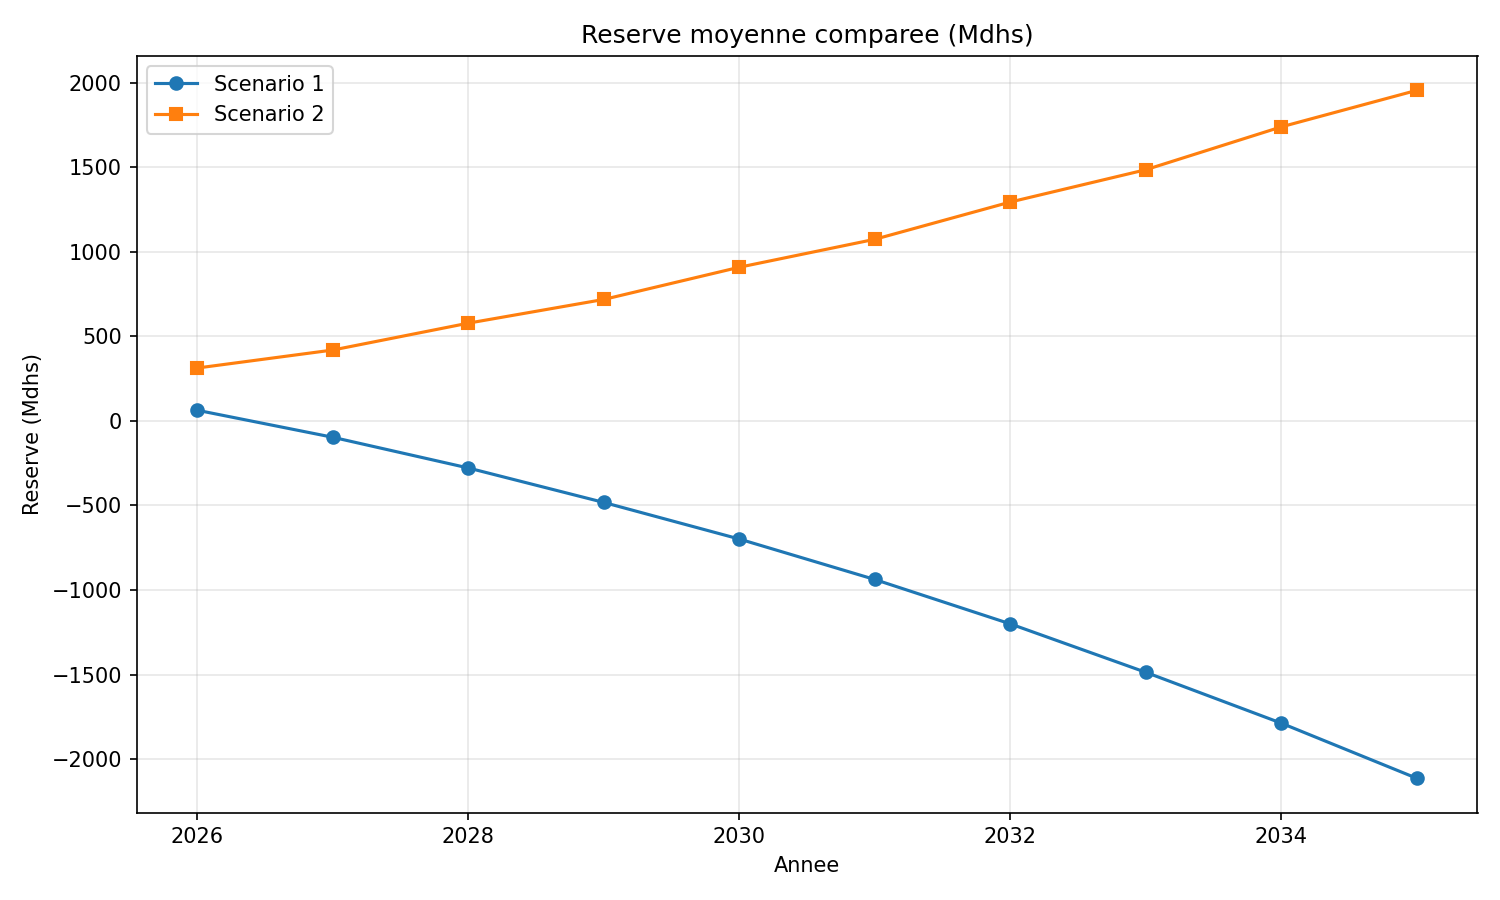
\includegraphics[width=0.9\linewidth]{graphique_01_reserve_comparee.png}
  \caption{Évolution de la réserve moyenne -- Scénario 1 vs Scénario 2.}
  \label{fig:reserve-cmp}
\end{figure}

\begin{figure}[H]
  \centering
  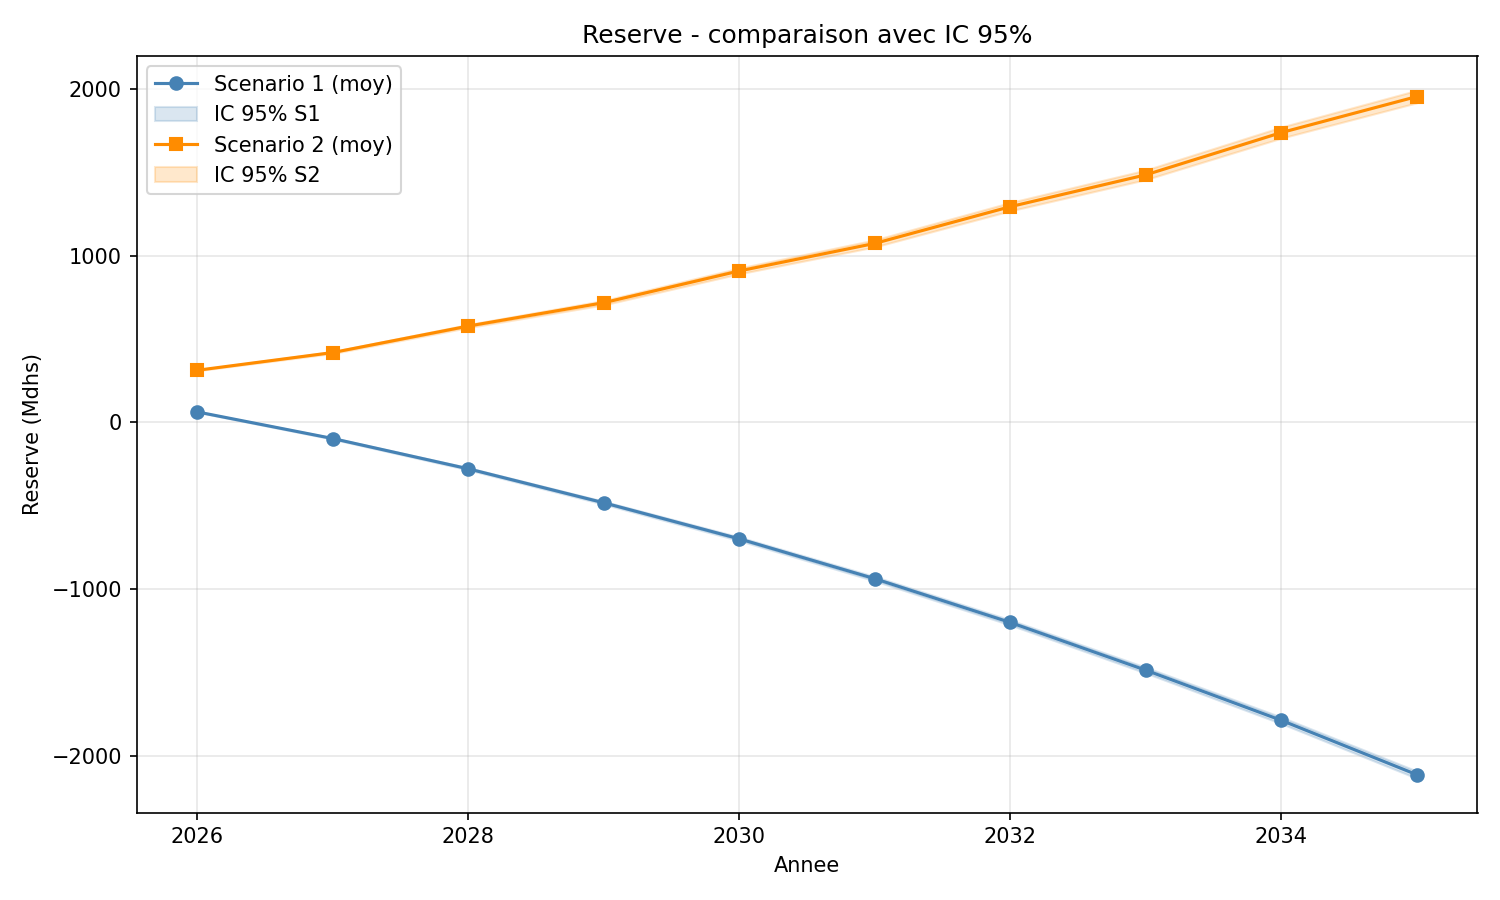
\includegraphics[width=0.9\linewidth]{graphique_10_comparaison_croisee.png}
  \caption{Réserve moyenne et IC à 95\,\% pour les deux scénarios.}
  \label{fig:reserve-ic}
\end{figure}

\begin{figure}[H]
  \centering
  \begin{subfigure}[t]{0.48\linewidth}
    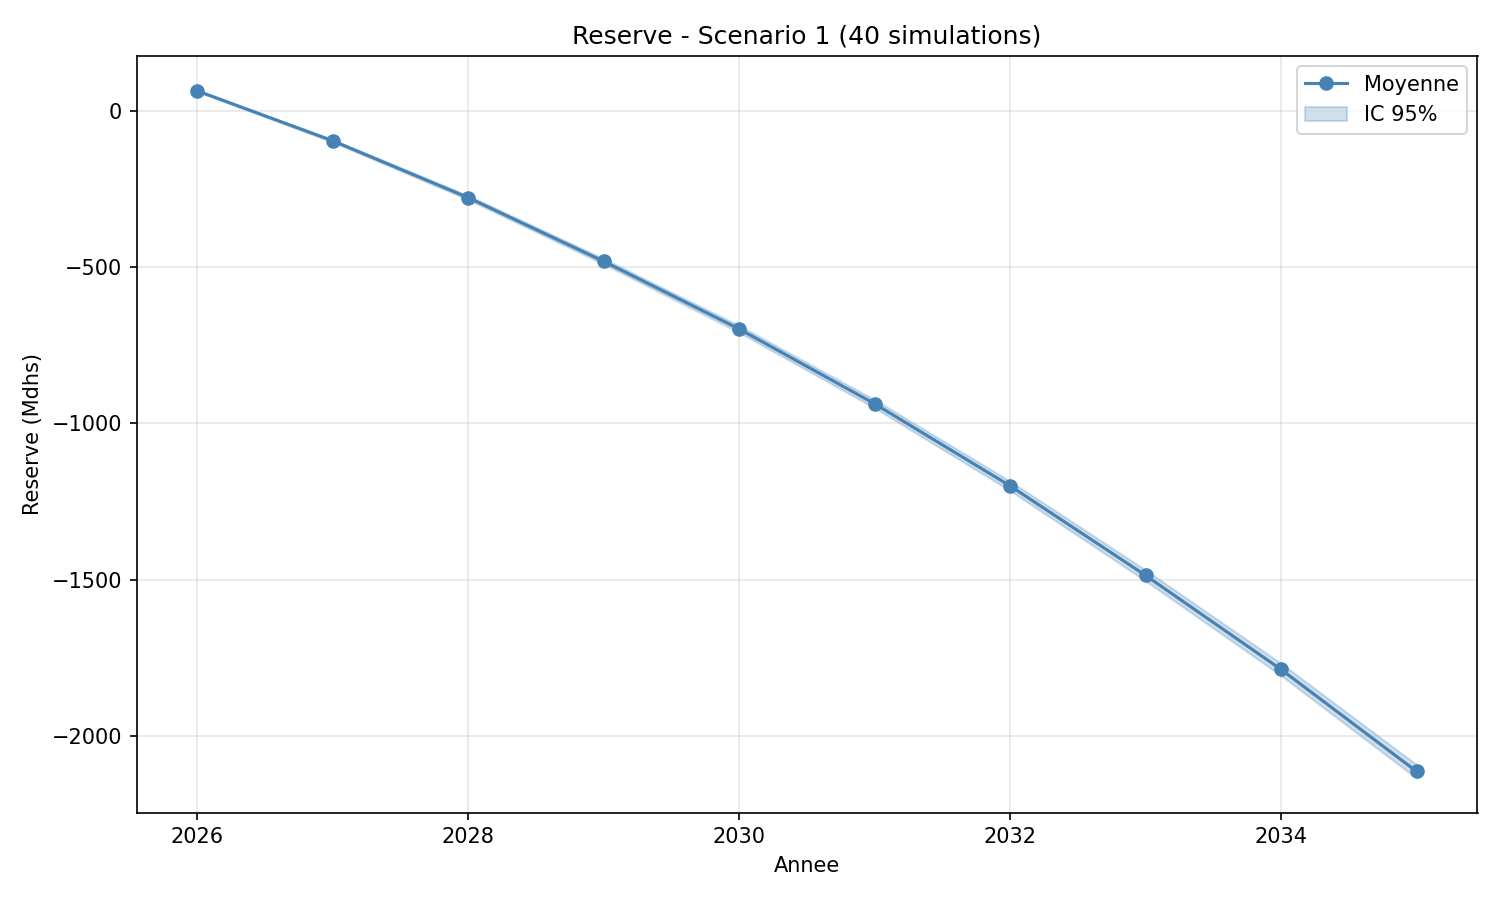
\includegraphics[width=\linewidth]{graphique_02_reserve_ic_scenario1.png}
    \caption{Réserve Scénario 1 avec IC.}
  \end{subfigure}\hfill
  \begin{subfigure}[t]{0.48\linewidth}
    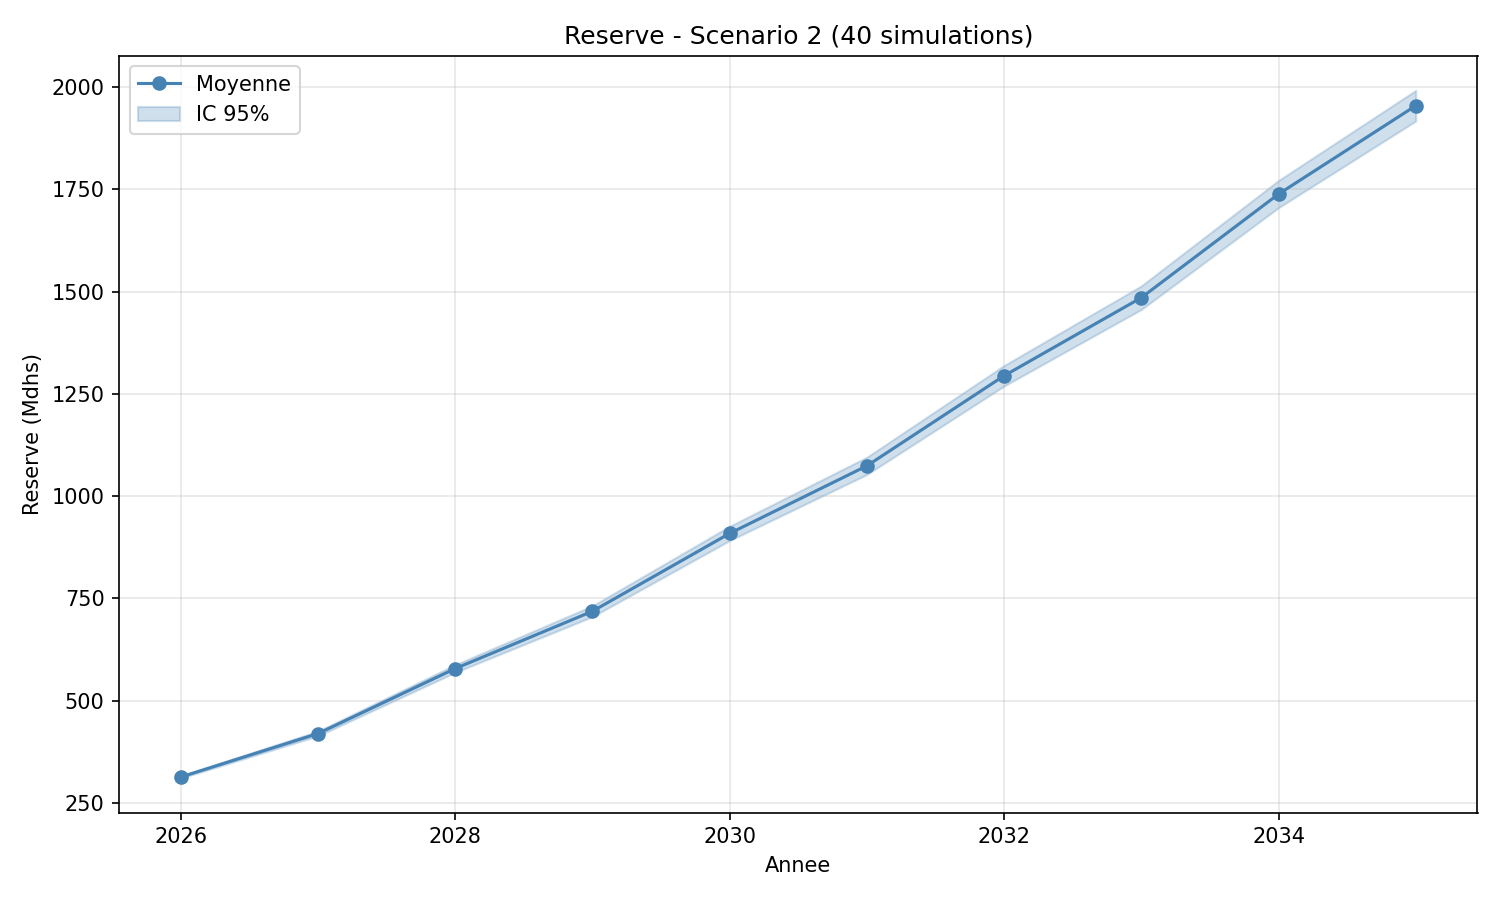
\includegraphics[width=\linewidth]{graphique_03_reserve_ic_scenario2.png}
    \caption{Réserve Scénario 2 avec IC.}
  \end{subfigure}
  \caption{Réserve par scénario avec bande d'IC à 95\,\%.}
\end{figure}

\begin{figure}[H]
  \centering
  \begin{subfigure}[t]{0.48\linewidth}
    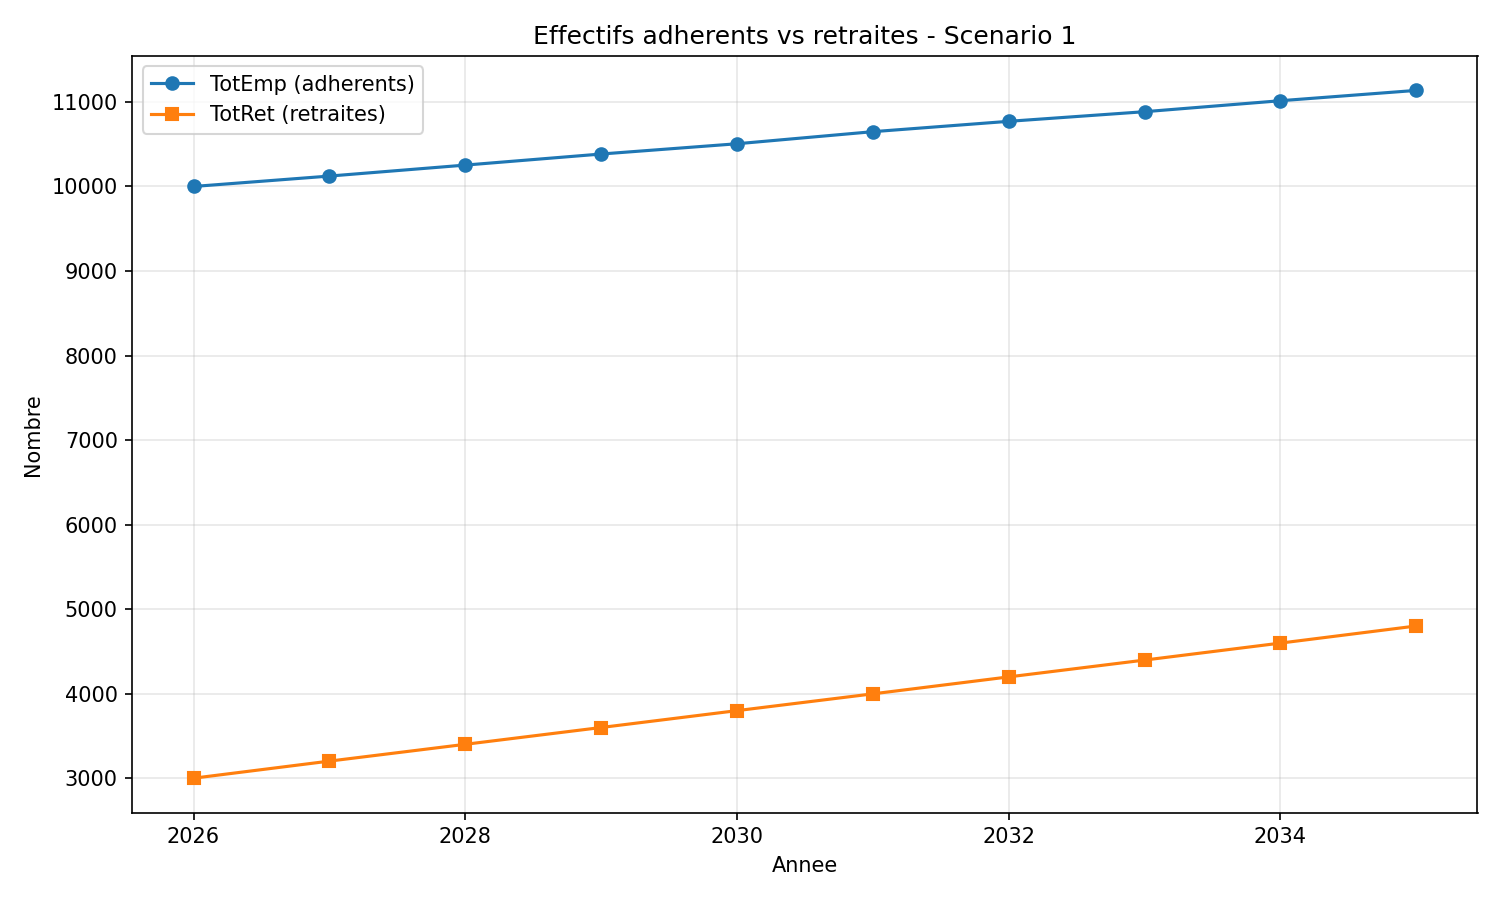
\includegraphics[width=\linewidth]{graphique_04_totemp_totret_s1.png}
    \caption{Effectifs Scénario 1.}
  \end{subfigure}\hfill
  \begin{subfigure}[t]{0.48\linewidth}
    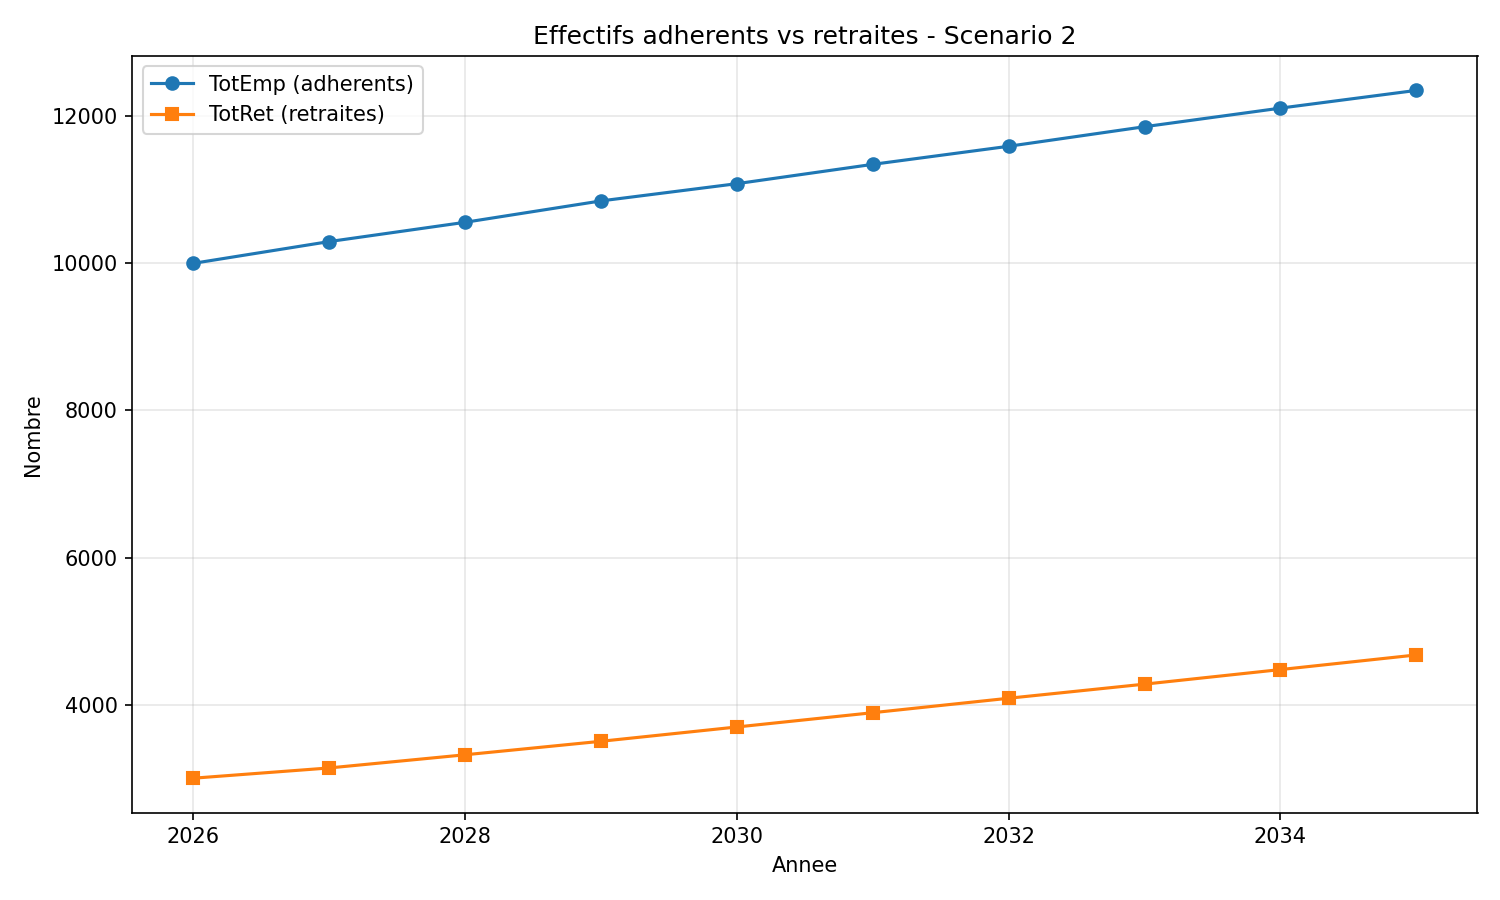
\includegraphics[width=\linewidth]{graphique_05_totemp_totret_s2.png}
    \caption{Effectifs Scénario 2.}
  \end{subfigure}
  \caption{Évolution des effectifs employés et retraités.}
\end{figure}

\begin{figure}[H]
  \centering
  \begin{subfigure}[t]{0.48\linewidth}
    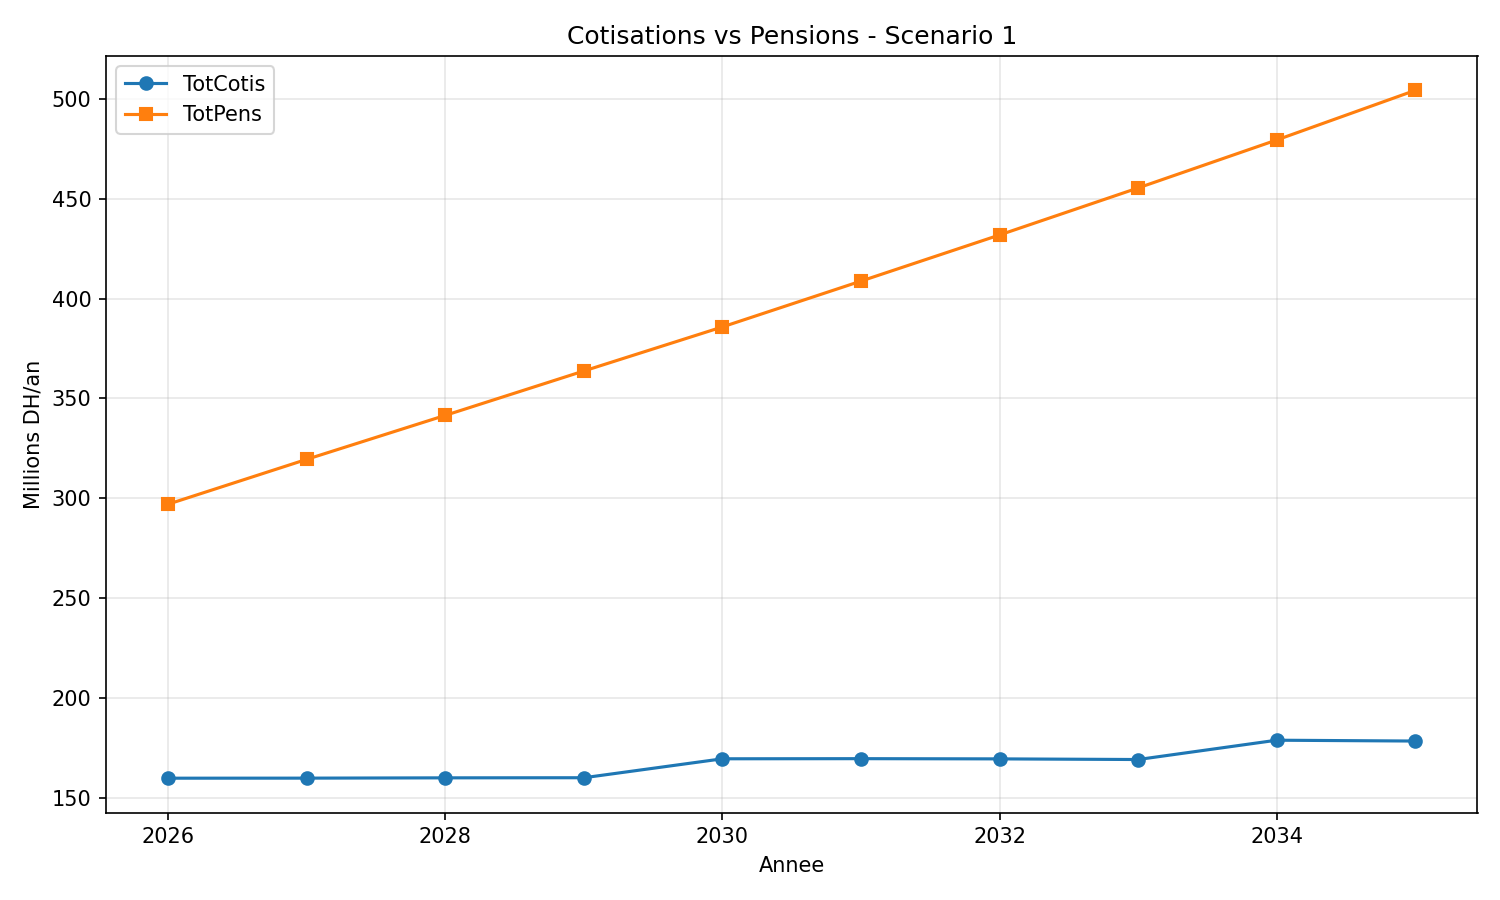
\includegraphics[width=\linewidth]{graphique_06_cotis_pens_s1.png}
    \caption{Cotisations vs Pensions -- S1.}
  \end{subfigure}\hfill
  \begin{subfigure}[t]{0.48\linewidth}
    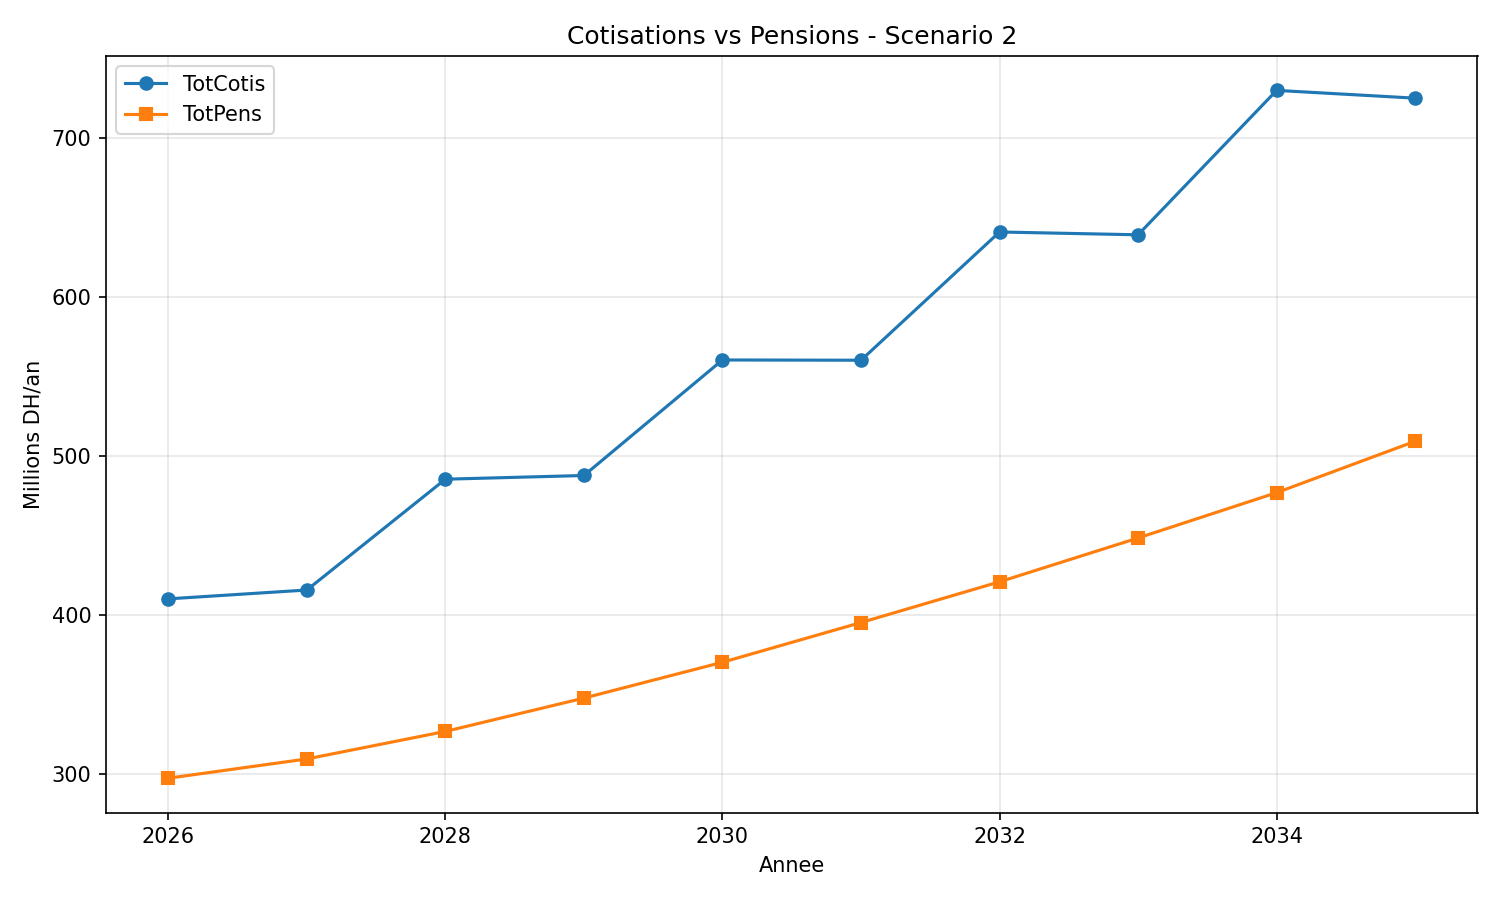
\includegraphics[width=\linewidth]{graphique_07_cotis_pens_s2.png}
    \caption{Cotisations vs Pensions -- S2.}
  \end{subfigure}
  \caption{Flux financiers annuels.}
\end{figure}

\begin{figure}[H]
  \centering
  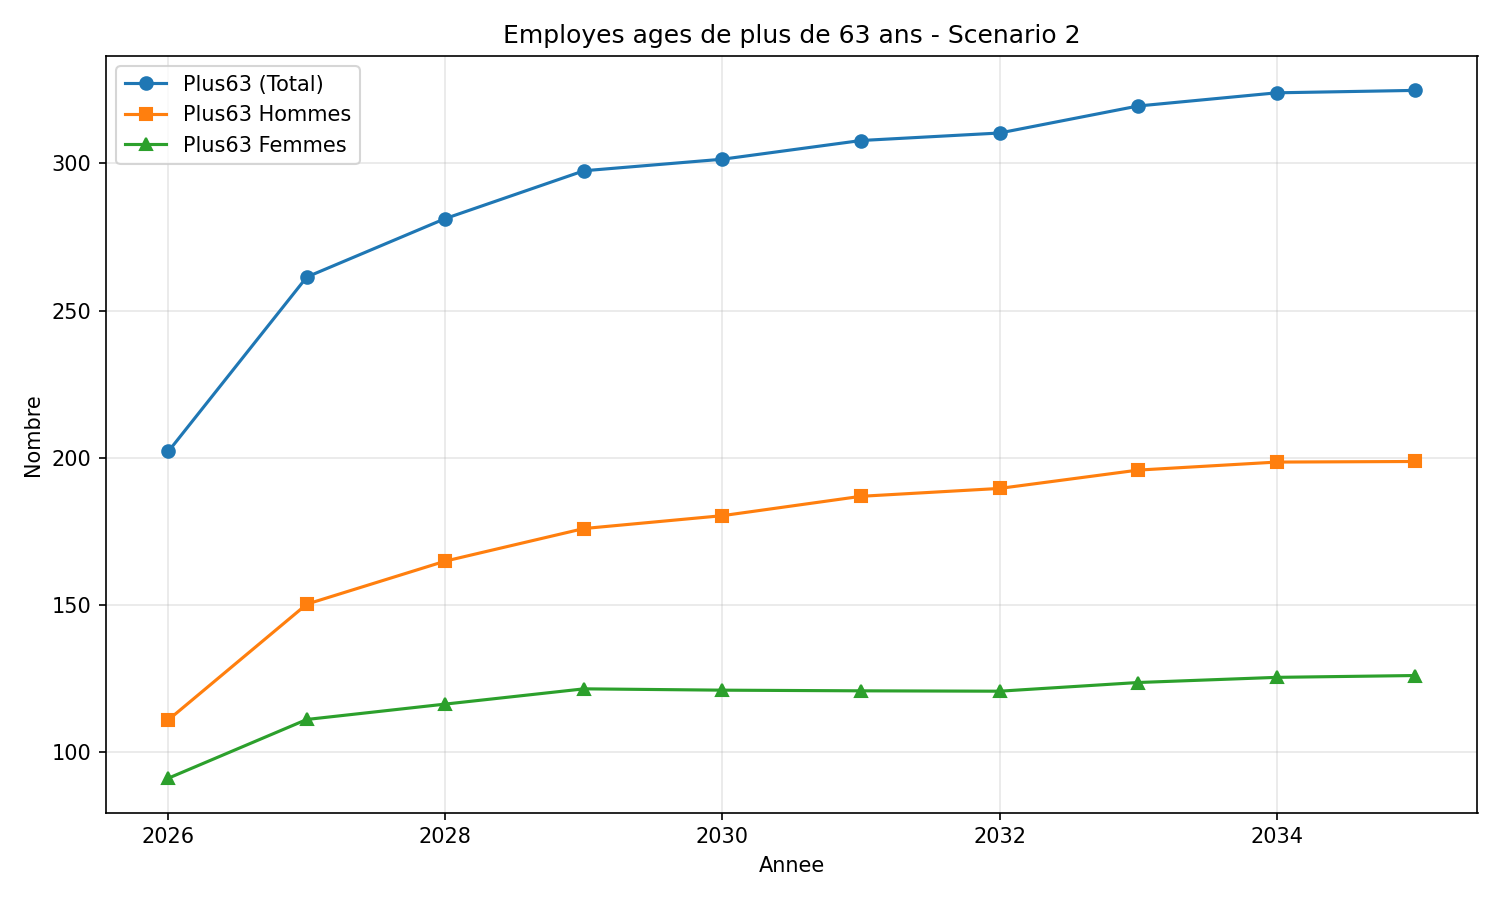
\includegraphics[width=0.8\linewidth]{graphique_08_plus63_evolution.png}
  \caption{Évolution des employés ayant prolongé au-delà de 63 ans
           (Scénario 2).}
\end{figure}

\begin{figure}[H]
  \centering
  \begin{subfigure}[t]{0.48\linewidth}
    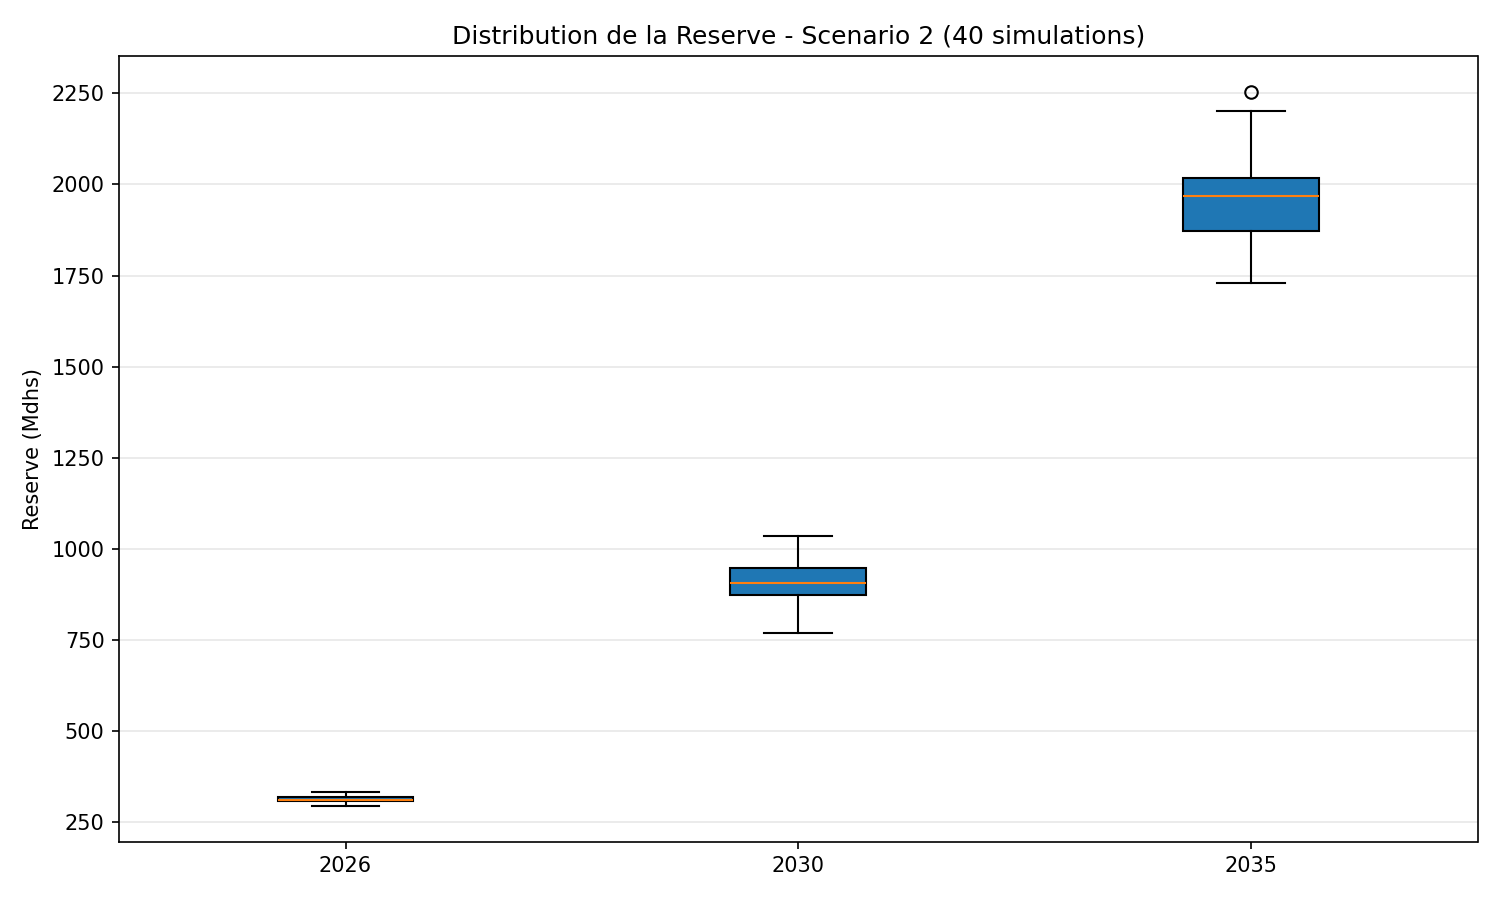
\includegraphics[width=\linewidth]{graphique_09_boxplot_reserve.png}
    \caption{Distribution de la Réserve.}
  \end{subfigure}\hfill
  \begin{subfigure}[t]{0.48\linewidth}
    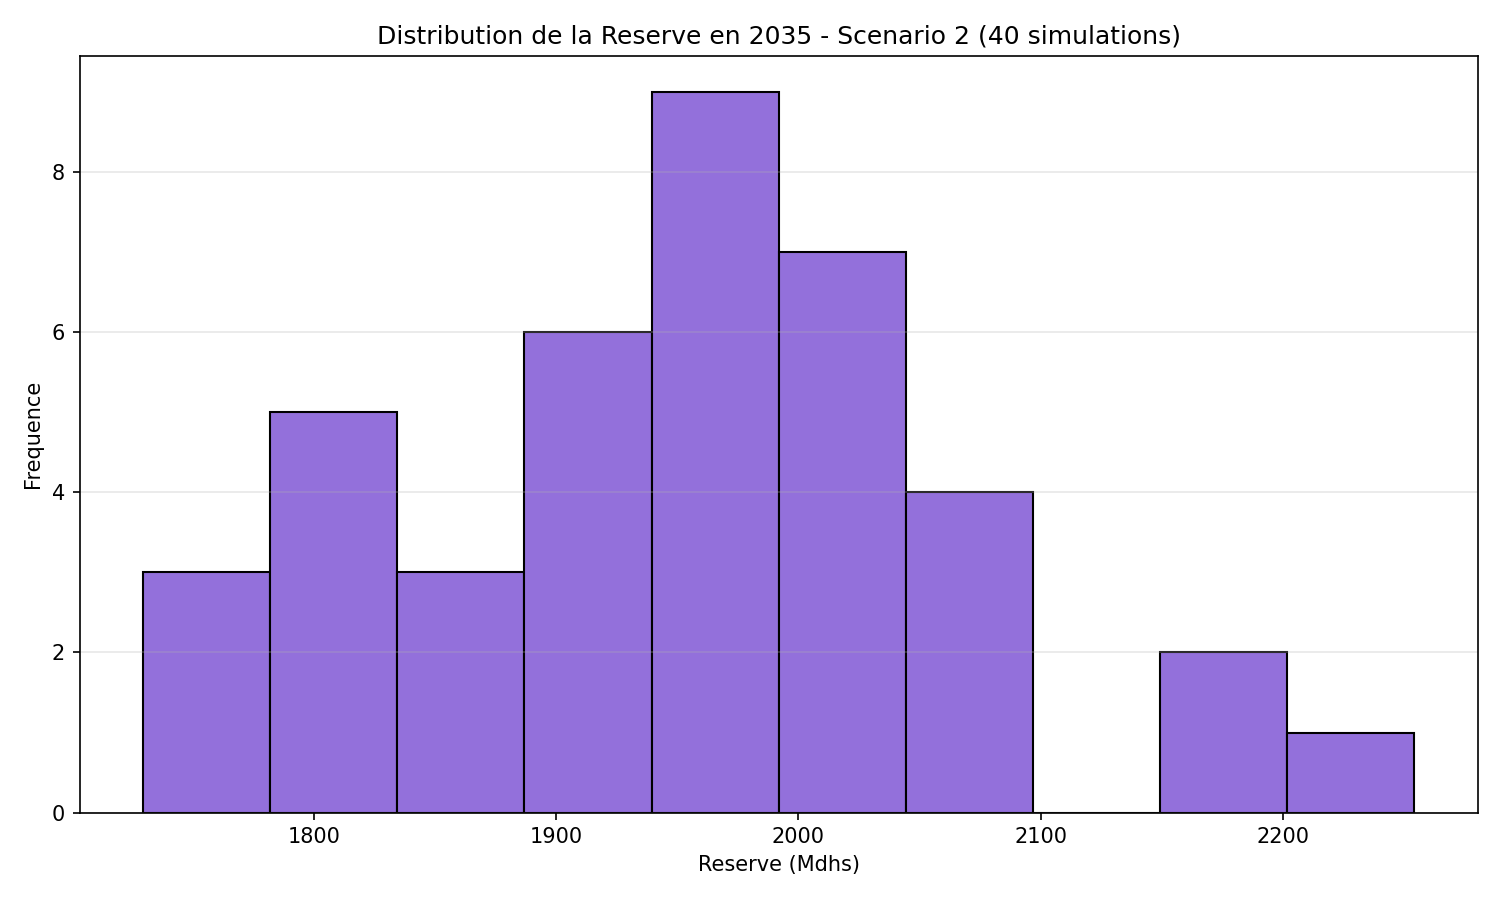
\includegraphics[width=\linewidth]{graphique_17_hist_reserve_2035.png}
    \caption{Histogramme Réserve 2035.}
  \end{subfigure}
  \caption{Analyse de la dispersion de la Réserve -- Scénario 2.}
\end{figure}

\section{Interprétation des résultats}

\subsection{Diagnostic du scénario actuel}

Le scénario de référence présente une \textbf{trajectoire de
ruine financière rapide} : la réserve devient négative dès 2027 et
atteint près de $-2{,}1$~milliards de dirhams en 2035. Cette dynamique
est imputable à trois facteurs combinés :
\begin{enumerate}
  \item Des taux de cotisation côté employé seul, plafonnés à 10\,\%,
        manifestement insuffisants.
  \item Un flux de nouveaux retraités stable (200--220 par an) face à un
        flux de cotisations qui ne progresse que par les avancements
        salariaux espacés.
  \item Un avancement modéré (+5\,\%) appliqué seulement trois fois sur
        la décennie.
\end{enumerate}

L'étroitesse des intervalles de confiance ($\approx 22$~Mdhs en 2035)
indique que cette conclusion est \textbf{très robuste} : le modèle est
peu sensible aux aléas de simulation, la trajectoire est essentiellement
déterministe.

\subsection{Apports de la réforme}

Le scénario de réforme inverse la tendance : la réserve atteint près de
$+1{,}95$~milliards de dirhams en 2035, soit un \textbf{écart cumulé de
plus de 4~milliards} par rapport au scénario actuel. Trois leviers
expliquent ce redressement :
\begin{itemize}
  \item le \textbf{doublement de la cotisation} par l'introduction d'une
        contribution employeur de même niveau que l'employé ;
  \item la \textbf{prolongation volontaire} d'une fraction des employés
        au-delà de 63 ans (300 à 325 personnes en moyenne en
        régime établi) qui continuent à cotiser au lieu de percevoir ;
  \item le \textbf{recrutement renforcé} (300--600 par an au lieu de
        250--400) qui élargit l'assiette de cotisation.
\end{itemize}

\subsection{Limites du modèle}

\begin{itemize}
  \item Absence de modélisation de la mortalité des retraités, ce qui
        \textbf{surévalue les pensions versées} et donc sous-estime
        l'écart en faveur de la réforme.
  \item Le rendement financier de la réserve (taux d'intérêt) n'est
        pas modélisé : la réserve est traitée comme un solde comptable
        sans capitalisation.
  \item L'horizon de 10 ans est court : les effets de la transition
        démographique sur 30--50 ans nécessiteraient un modèle élargi.
\end{itemize}

\section{Conclusion du chapitre}

L'expérimentation confirme l'urgence d'une réforme paramétrique. Au-delà
des chiffres bruts, les intervalles de confiance étroits attestent de la
robustesse statistique des résultats : sur 40 simulations indépendantes,
aucune ne montre de scénario favorable au régime actuel.

% ============================================================================
\chapter*{Conclusion Générale}
\addcontentsline{toc}{chapter}{Conclusion Générale}
% ============================================================================

Ce projet a permis de mettre en œuvre une simulation discrète complète
d'un système de retraite par répartition inspiré du régime de la fonction
publique marocaine, en respectant l'ensemble des contraintes
méthodologiques imposées par le sujet : générateur de Wichmann-Hill,
distributions empiriques, structures de données en mémoire, et calcul
d'intervalles de confiance sur 40 simulations indépendantes.

Sur le plan \textbf{technique}, l'architecture modulaire (11~modules
Python distincts) a permis une séparation claire des responsabilités et
facilité le développement incrémental. Le double point d'entrée -- CLI
et tableau de bord Streamlit -- offre à la fois une utilisation
scriptable pour la production de rapports et une exploration interactive
des résultats.

Sur le plan des \textbf{résultats}, l'étude conclut sans ambiguïté à la
\textbf{non-viabilité du régime actuel} sur l'horizon 2026--2035 : la
faillite survient dès la deuxième année et le déficit cumulé atteint
2,1~milliards de dirhams. La réforme paramétrique proposée
(cotisation partagée, départ flexible 63--70 ans, avancement renforcé,
recrutement augmenté) renverse complètement la trajectoire et permet de
constituer une réserve excédentaire de près de 2~milliards.

Plusieurs \textbf{perspectives} d'extension sont envisageables :
\begin{itemize}
  \item intégration d'un modèle de mortalité (tables actuarielles
        marocaines) ;
  \item prise en compte du rendement financier de la réserve ;
  \item modélisation de chocs économiques (récession, inflation forte) ;
  \item extension de l'horizon à 30 ans pour mesurer l'impact de la
        transition démographique de long terme ;
  \item couplage avec des données réelles de la CMR pour calibrer les
        distributions.
\end{itemize}

Au-delà du résultat chiffré, ce projet illustre la valeur de la
simulation discrète comme \textbf{outil d'aide à la décision publique}
pour des systèmes complexes où l'expérimentation réelle est impossible.

% ============================================================================
\addcontentsline{toc}{chapter}{Bibliographie}
\begin{thebibliography}{99}

\bibitem{wichmann}
B. A. Wichmann et I. D. Hill, \emph{Algorithm AS 183: An Efficient and
Portable Pseudo-Random Number Generator}, Applied Statistics, vol. 31,
n\textsuperscript{o} 2, p. 188-190, 1982.

\bibitem{law-kelton}
A. M. Law, \emph{Simulation Modeling and Analysis}, 5\textsuperscript{e}
édition, McGraw-Hill, 2014.

\bibitem{ross-simulation}
S. M. Ross, \emph{Simulation}, 5\textsuperscript{e} édition,
Academic Press, 2012.

\bibitem{cmr}
Caisse Marocaine des Retraites, \emph{Rapport annuel d'activité 2023},
Rabat, 2024.

\bibitem{ocde-pensions}
OCDE, \emph{Pensions at a Glance 2023 -- OECD and G20 Indicators},
Éditions OCDE, Paris, 2023.

\bibitem{python-doc}
Python Software Foundation, \emph{The Python Language Reference --
version 3.10}, \url{https://docs.python.org/3.10/}, consulté en 2026.

\bibitem{matplotlib}
J. D. Hunter, \emph{Matplotlib: A 2D Graphics Environment}, Computing in
Science \& Engineering, vol. 9, n\textsuperscript{o} 3, p. 90-95, 2007.

\bibitem{streamlit}
Streamlit Inc., \emph{Streamlit Documentation},
\url{https://docs.streamlit.io/}, consulté en 2026.

\bibitem{numpy}
C. R. Harris \emph{et al.}, \emph{Array programming with NumPy}, Nature,
vol. 585, p. 357-362, 2020.

\end{thebibliography}

\end{document}
